\question
(0,5 балла) Василина всегда любила приезжать летом к бабушке и собирать с ней ягоды в лесу. Сегодня же бабушка занята, а Василине придется самой разобраться с картой всех тропинок и опушек.

\begin{minipage}[h]{0.45\linewidth}
\center{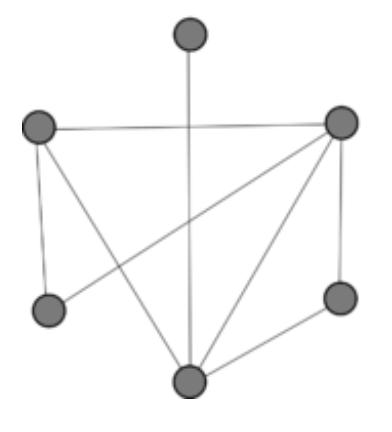
\includegraphics[width=0.4\textwidth]{pic/88.jpg} }
\end{minipage}

\begin{enumerate}
    \item Выясните, сможет ли Василина пройти по всем тропинкам один раз и вернуться на исходную опушку?
    \item Сможет ли Василина обойти все опушки по одному разу?
    \item Можно ли перерисовать карту так, чтобы ни одна тропинка не пересекалась с другой?
\end{enumerate}
Подробно опишите и докажите свои рассуждения.

---------------

Автор -- София Рахматуллина